
\section{Neuartige Antriebe}
Bei der Wahl den alternativen Antrieben sind bestimmte Überlegungen relevant. welcher volumetrische und gravimetrische Energie, Kosten 
und Verfügbarkeit des Rohstoffs, Sicherheit in Bezug auf Herstellung und Benutzung, 
direkte und indirekte \ce{CO2} Emissionen \cite{ansell2023review}.



In diesem Kapitel werden folgende vielversprechende Energieträger angeschaut und zusammengefasst: nachhaltige Kraftstoffe (SAF), 
Batterie-Antriebe (elektrochemische) und Wasserstoff.



\subsection{Sustainable Aviation Fuel (SAF)}

Sustainable Aviation Fuel oder nachhaltige Flugtreibstoff sind synthetische flüssige Biotreibstoffe oder renewable non-biological sources, 
die mit herkömmlichem Flugkraftstoff und bestehenden Betankungssysteme kompatibel sind. Deswegen werden sie auch als Drop-In Treibstoff bezeichnet
\cite{iata_saf_2024}. IATA besagt, dass die zulässige Mischrate zurzeit max. 50 \% beträgt. Meisten SAF weisen keine Aromaten auf, 
fehlende/andere aromatische Gehalt in den SAF kann zu Leckagen in der Dichtung führen \cite{jarin2024emissions}. 
Bis jetzt ist kein Flugzeug für das Fliegen mit reinem SAF zertifiziert \cite{iata_saf_2024}, 
allerdings bereits im November 2023 hat der Fluggesellschaft Virgin Atlantic den ersten transatlantischen Demonstrationsflug 
(mit einem Boeing 787) mit 100 \% SAF (88 \%HEFA und 12\% Synthetic Aromatic Kerosene (SAK) ) durchgeführt \cite{virginatlantic_saf_2023}.
Das bringt die Hoffnung, dass Reduktion von CO2 mit dieser Vorgehensweise realisiert werden kann. Die manchen Fluggesellschaften nutzen jetzt
geblendete SAFs (Quelle). 

Es gibt elf Verfahren für SAF-Produktion, dafür werden verschiedene Rohstoffe benutze, beispielsweise Algen, Biomasse oder Kohle 
genutzt und bis jetzt gibt es kein alternativer Flugtreibstoff, die Emissionen komplett vermeidet. \cite{icao_saf_conversion_2024}.

Biofuels: keine änderung in flugzeug oder betankungssystem notwendig \cite{sky2020hydrogen}.

Die vier wichtigsten Technologie sind Hydroprocessed Esters and Fatty Acids (HEFA), Fischer-Tropsch (FT), Alcohol to Jet (ATJ) 
und Power to Liquid (PtL). Bis jetzt nur HEFA kommerziell zugelassen.

In der Abbildung XX sind die SAF Produktionswege aus unterschiedlichen Quellen aufgelistet und den Teil des Kohlenstoffdioxids,
die mit diesen Wegen reduziert werden. Bemerkenswert ist, dass die Herstellung
aus einer Kombination aus Kohlenmonoxid (CO) und Wasserstoff (H2) durch das katalytische Verfahren nach Fischer-Tropsch (existing renewables), 
auch PtL genannt, fast bis 100 \% CO2-Ausstoß reduziert, gefolgt von Municipal Solid Waste (MSW). 
Herstellung nach der FT-Technologie zeigt die größten Emissionseinsparungen \cite{iata_saf_2024, de2017life}.

PtL: brauche ich das überhaupt?
CO2 kann durch Direct Air Capture (DAC) aus der Luft gewonnen werden und dann mittels 
Reverse-Water-Gas-Shift-Reaktion (RWGS) mit Wasserstoff zu CO2 umgewandelt werden. 
PtL ist sehr energieintensiv und braucht erneuerbare Stromquelle (hängt davon ab).
\cite{ansell2023review}
Eine Herausforderung im Blick auf Ressourcen- und Flächenbedarf bleibt bei biogenen oder PtL-Synthese \cite{ansell2023review}.

MSW ist Abfall aus nicht biogenen Quellen, wie Kunststoffe. \cite{icao_saf_conversion_2024} PtL SAF "Trotz der erheblichen Herausforderungen 
bietet sich PtL SAF an, langfristig einer der stärksten Beiträge zur Energiewende der Fluggesellschaften zu werden."

Kosten:
https://www.icao.int/environmental-protection/Pages/SAF_RULESOFTHUMB.aspx
https://theicct.org/sites/default/files/publications/Alternative_jet_fuels_cost_EU_20190320_1.pdf
"Overall, estimates of capital spending
on renewable diesel/HEFA facilities
ra n g e f ro m a ro u n d € 0. 4 0 to
€1.50 per liter of annual capacity,
averaging around €0.60 per liter,
with larger facilities generally having
lower per-liter capital costs due to
economies of scale"
ICAO hat eine Reihe von Heuristiken rausgebracht, um Preisschätzungen unter SAF-Kraftstoffen zu ermitteln. (für USA)
FT mit Feedstock CO2 from Direct Air Capture, H2 - Feedstock Price \$300/t, \$6/kg, Total capacity 1000 mill L/year.
FT aus MSW - \$30/ton 

Diese Arbeit wird auf reine SAF ohne Beimischung beschränkt, da nur so kann das Ziel 2050 erreicht werden. 
Deswegen werden im Weiteren die alternativen Luftfahrzeugkonzepte angeschaut, die Beförderung mit SAF realistisch machen.


Infrastruktur: Das reine SAF wurde noch nicht zertifiziert, um in das Treibstofflager vom Flughafen zu gelangen \cite{iata_saf_2024}.

%Im März 2024 hat International Aero Engines AG (IAE) bei der MTU Maintenance ein V2500-Triebwerk mit 100 \% nachhaltigem 
%Flugkraftstoff HEFA-SPK getestet.

Die Preise für nachhaltige Flugtreibstoffe sind zwei- bis zu fünfmal höher als für herkömmliche Kerosin. (viel kleinere Nachfrage bis jetzt)

Einbindung in Regularien

In EU-Richtlinien sowie in CORSIA sind die Kriterien für SAF-Qualität festgelegt.

Im Rahmen EU-ETS gelten SAFs als emissionsfrei und bei der richtigen Zertifizierung sind vor der Abgabe von CO2-Zertifikaten 
befreit \cite{icao_saf_conversion_2024}. Um Fluggesellschaften für die Nutzung der nachhaltigen Kraftstoffe zu motivieren/anreizen, hat EU-ETS
20 Mio Zertifikaten zur Verfügung gestellt \cite{icao_saf_conversion_2024}.

In der CORSIA 


\begin{figure}[h]
	\centering
	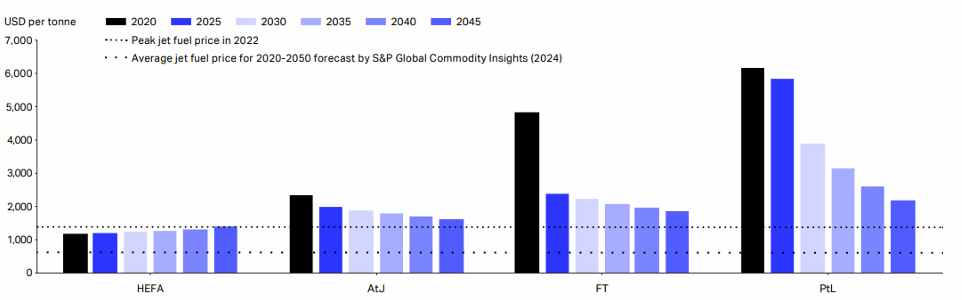
\includegraphics[width=0.4\linewidth]{Bilder/Preise SAF.png}
	\caption[Durchschnittlicher IATA-Mindestverkaufspreis (MSP) der wichtigsten SAF-Pfade über den Zeitraum 2020 bis 2050]{Durchschnittlicher IATA-Mindestverkaufspreis \cite{icao_saf_conversion_2024}}
	\label{fuelcell}
\end{figure}

HEFA ist die fortgeschrittenste Technologie im SAF-Markt.

K. Dahal "Current 
engine and propulsion systems are not compatible with 100 \% bio-jet 
fuels which require retrofitting and development of new engine pro
pulsion systems. "

\cite{mensen2013handbuch}  "Im Bereich Kraftstoffverbrauch und Lärm wurde in den letzten 30 Jahren bereits 
Reduktion von ca. 50 \% bzw. 20 dB erzielt."


Nach ASTM D7566 müssen Kraftstoffe einen bestimmten Gehalt an Aromaten aufweisen, um kompatibel mit ben bestehenden Flugzeugen zu sein. (Quelle?)

Quelle: Synthetic aromatic kerosene property prediction improvements with isomer specific characterization via GCxGC 
and vacuum ultraviolet spectroscopy: 
SAK besteht grundlegend aus Aromaten und unterscheidet sich deutlich von den anderen SAFs und wird für Aufschwellung von Dichtungen. 
"Aromaten sind organische Verbindungen, die die Schmierfähigkeit, Dichte und Materialverträglichkeit des Flugkraftstoffs verbessern"

Die sind gleichzeitig für Kondensstreifen verantwortlich (Quelle), die klimanegativ wirken (Quelle). 
Also die ersten rein SAF-Flüge werden nicht null emissionsfrei sein.

Derzeit wird von ASTM evaluiert \cite{icao_saf_conversion_2024}.
HEFA und SAK Mischung können die 100\% SAF-Flüge ermöglichen, dabei reduziert die Mischung die Rußpartikeln.

Laut IATA durch Drop-In SAF können die Emissionen um 62 \% reduziert werden. https://www.iata.org/en/pressroom/2023-releases/2023-06-04-03/
"As a drop-in solution, SAF is expected to deliver about 62\% of carbon mitigation needed to achieve net zero by 2050"

Manche berichten, dass Flugdistanz bei SAF gleich(Quelle), und dazu machen zum Schluss gekommen, dass 
Treibstoffverbrauch verringert werden kann(Quelle).
Annahme: Verbrauch bei konventionellen und SAF gleich

